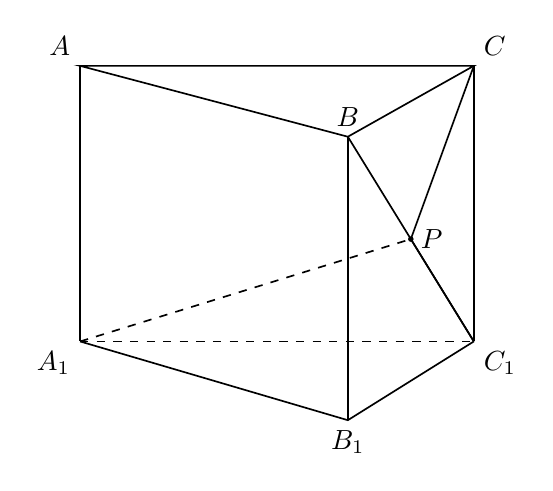
\begin{tikzpicture}[line width=.6pt]
\coordinate (A) at (0.0,4.5);
\coordinate (C) at (5.0,4.5);
\coordinate (B) at (3.4,3.6);
\coordinate (A1) at (0.0,1.0);
\coordinate (C1) at (5.0,1.0);
\coordinate (B1) at (3.4,0.0);
\coordinate (P) at (4.2,2.3);
% top and bottom faces
\draw (A)--(B)--(C)--cycle;
\draw (A1)--(B1)--(C1);
\draw[dashed] (A1)--(C1);
% verticals
\draw (A)--(A1);
\draw (B)--(B1);
\draw (C)--(C1);
% point P on BC1 and segments
\draw (B)--(C1);
\draw (C)--(P)--(C1);
\draw[dashed] (A1)--(P);
\fill (P) circle (1.0pt);
\node[above left] at (A) {$A$};
\node[above right] at (C) {$C$};
\node[above] at (B) {$B$};
\node[below left] at (A1) {$A_{1}$};
\node[below right] at (C1) {$C_{1}$};
\node[below] at (B1) {$B_{1}$};
\node[right] at (P) {$P$};
\end{tikzpicture}
